%%***********************************************
%% Plantilla para TFG.
%% Escuela Técnica Superior de Ingenieros Informáticos. UPM.
%%***********************************************
\documentclass[a4paper,11pt, hidelinks]{book}
%%-----------------------------------------------
%% Importar Preámbulo:
% -*-coding: utf-8 -*-
%%***********************************************
%% Plantilla para TFG.
%% Escuela Técnica Superior de Ingenieros Informáticos. UPM.
%%***********************************************
%% Preámbulo del documento.
%%***********************************************
\usepackage[utf8]{inputenc}
\usepackage[T1]{fontenc}
\usepackage[english,spanish,es-lcroman]{babel}
\usepackage{bookman}
\decimalpoint
\usepackage{graphicx}
\usepackage{bookmark}
\usepackage{amsfonts,amsgen,amsmath,amssymb}
\usepackage[top=3cm, bottom=3cm, right=2.54cm, left=2.54cm]{geometry}
\usepackage{afterpage}
\usepackage{colortbl,longtable}
\usepackage{hyperref} 
\usepackage{pdfpages}
\usepackage{url}
\usepackage{multicol}
\usepackage[stable]{footmisc}
\usepackage{parskip} % para separar párrafos con espacio.
%%-----------------------------------------------
\usepackage{fancyhdr}
\pagestyle{fancy}
\fancyhf{}
\fancyhead[LO]{\leftmark}
\fancyhead[RE]{\rightmark}
\setlength{\headheight}{1.5\headheight}
\cfoot{\thepage}

\addto\captionsspanish{ \renewcommand{\contentsname}
  {Tabla de contenidos} }
\setcounter{tocdepth}{4}
\setcounter{secnumdepth}{4}

\renewcommand{\chaptermark}[1]{\markboth{\textbf{#1}}{}}
\renewcommand{\sectionmark}[1]{\markright{\textbf{\thesection. #1}}}
\newcommand{\HRule}{\rule{\linewidth}{0.5mm}}
\newcommand{\bigrule}{\titlerule[0.5mm]}

\usepackage{appendix}
\renewcommand{\appendixname}{Anexos}
\renewcommand{\appendixtocname}{Anexos}
%\renewcommand{\appendixpagename}{Anexos}
%%-----------------------------------------------
%% Páginas en blanco sin cabecera:
%%-----------------------------------------------
\usepackage{dcolumn}
\newcolumntype{.}{D{.}{\esperiod}{-1}}
\makeatletter
\addto\shorthandsspanish{\let\esperiod\es@period@code}

\def\clearpage{
  \ifvmode
    \ifnum \@dbltopnum =\m@ne
      \ifdim \pagetotal <\topskip
        \hbox{}
      \fi
    \fi
  \fi
  \newpage
  \thispagestyle{empty}
  \write\m@ne{}
  \vbox{}
  \penalty -\@Mi
}
\makeatother
%%-----------------------------------------------
%% Estilos código de lenguajes: Consola, C, C++ y Python
%%-----------------------------------------------
\usepackage{xcolor}

\definecolor{gray97}{gray}{.97}
\definecolor{gray75}{gray}{.75}
\definecolor{gray45}{gray}{.45}

\usepackage{listings}
\lstset{ frame=Ltb,
     framerule=0pt,
     aboveskip=0.5cm,
     framextopmargin=3pt,
     framexbottommargin=3pt,
     framexleftmargin=0.4cm,
     framesep=0pt,
     rulesep=.4pt,
     backgroundcolor=\color{gray97},
     rulesepcolor=\color{black},
     %
     stringstyle=\ttfamily,
     showstringspaces = false,
     basicstyle=\scriptsize\ttfamily,
     commentstyle=\color{gray45},
     keywordstyle=\bfseries,
     %
     numbers=left,
     numbersep=6pt,
     numberstyle=\tiny,
     numberfirstline = false,
     breaklines=true,
   }
\lstnewenvironment{listing}[1][]
   {\lstset{#1}\pagebreak[0]}{\pagebreak[0]}

\lstdefinestyle{consola}
   {basicstyle=\scriptsize\bf\ttfamily,
    backgroundcolor=\color{gray75},    
    }

\lstdefinestyle{CodigoC}
   {basicstyle=\scriptsize,
	frame=single,
	language=C,
	numbers=left
   }
   
\lstdefinestyle{CodigoC++}
   {basicstyle=\small,
	frame=single,
	backgroundcolor=\color{gray75},
	language=C++,
	numbers=left
   }

\lstdefinestyle{Python}
   {language=Python,    
   }

\lstdefinelanguage{yaml}
{
   keywords={true,false,null,y,n},
   keywordstyle=\bfseries,
   basicstyle=\bfseries,
   sensitive=false,
   captionpos=b,
   comment=[l]{\#},
   morecomment=[s]{/*}{*/},
   commentstyle=\ttfamily,
   stringstyle=\mdseries\ttfamily,
   moredelim=[l]{\&},
   moredelim=[l]{*},
   moredelim=**[il][\mdseries{:}\mdseries]{:},
   morestring=[b]',
   morestring=[b]",
   literate =  {---}{{\llap{\mdseries-{-}-}}}3    
               {|}{{\textbar}}1 
               {\ -\ }{{\mdseries\ -\ }}3,
}

\colorlet{punct}{red!60!black}
\definecolor{delim}{RGB}{20,105,176}
\colorlet{numb}{magenta!60!black}
\lstdefinelanguage{json}{
   basicstyle=\bfseries,
   captionpos=b,
   showstringspaces=false,
   breaklines=true,
   stringstyle=\mdseries\ttfamily,
   moredelim=[l]{\&},
   moredelim=[l]{*},
   moredelim=**[il][\mdseries{:}\mdseries]{:},
   morestring=[b]',
   morestring=[b]",
   frame=lines
}

\usepackage[textwidth=2.5cm, textsize=smaller]{todonotes}
\setlength{\marginparwidth}{2.5cm}

\usepackage{lipsum}

\usepackage{relsize}

%%-----------------------------------------------
%% Cargar datos relativos al TFG:
%% (actualizar estos datos en secciones/_DatosTFG.tex) 
%%***********************************************
%% Plantilla para TFG.
%% Escuela Técnica Superior de Ingenieros Informáticos. UPM.
%%***********************************************
%% Información requerida para completar la portada.
%%*********************************************** 

%% Escribe Nombre y Apellidos del autor del trabajo:
\newcommand{\NombreAutor}{ Arturo Vidal Peña }

%% Escribe el Grado: 
\newcommand{\Grado}{ Grado en Ingeniería Informática }

%% Escribe el Título del Trabajo:
\newcommand{\TituloTFG}{ Grafana, Alert-Manager and Prometheus Manager } 

%% Escribe Nombre y Apellidos del Tutor del trabajo: 
\newcommand{\NombreTutor}{ Pérez Costoya, Fernando } 

% Escribe el Departamento al que pertenece el Tutor:
\newcommand{\Departamento}{\parbox{\dimexpr\linewidth-53\fboxsep}{ Departamento de Arquitectura y Tecnología de Sistemas Informáticos }}

% Escribe la fecha de lectura, en formato: Mes - Año
\newcommand{\Fecha}{ Junio  2022 }
%%***********************************************

% Empresa colaboradora:
\newcommand{\EmpresaColaboradora}{Accenture Technologies S.L.}

%%-----------------------------------------------
%% Documento:
\begin{document}
%%***********************************************
%% Plantilla para TFG.
%% Escuela Técnica Superior de Ingenieros Informáticos. UPM.
%%***********************************************
%% Portada. 
%%***********************************************
\begin{titlepage}

\begin{minipage}{0.15\linewidth}
\hspace*{-2.5cm}
\noindent

\includegraphics[scale=0.5]{include/EscUpm.png} \qquad\qquad
\end{minipage}
\begin{minipage}{0.7\linewidth}
\begin{center}
\huge{ Universidad Politécnica\\de Madrid }\\
\vspace*{0.5cm}
\Large{\textbf{Escuela Técnica Superior de \\
Ingenieros Informáticos}}
\end{center}
\end{minipage}
\begin{minipage}{0.2\linewidth}

\includegraphics[scale=0.5]{include/FacInformatica.png} 
\end{minipage}

\vspace*{1cm}
\begin{center}
\Large{Grado en  \Grado{} }
\end{center}

\vspace*{1cm}
\begin{center}
\huge{ Trabajo Fin de Grado }
\end{center}

\vspace*{0.5cm}
\begin{center}
\huge\bfseries {  \TituloTFG{} } 
\end{center}

\vspace*{5cm}

\noindent
\large{Autor: \NombreAutor{} }\\
\large{Tutor(a): \NombreTutor{} }\\
\large{Empresa colaboradora: \EmpresaColaboradora{} }


\vspace*{4cm}
\begin{center}
Madrid, \Fecha
\end{center}

%%--------------------------------
\newpage
\thispagestyle{empty}
%%--------------------------------
\noindent
Este Trabajo Fin de Grado se ha depositado en la ETSI Informáticos de la Universidad Politécnica de Madrid para su defensa.

\vspace*{4cm}
\noindent
\textit{Trabajo Fin de Grado}\\
\textit{Grado en} \Grado{}

\begin{enumerate}
\item[\textit{Título:}] \TituloTFG{}
\end{enumerate}
\Fecha


\vspace*{3cm}

\noindent
\begin{tabular}{ll}
\textit{Autor:} & \NombreAutor{}  \\ 
\textit{Tutor:} & \NombreTutor{}  \\ 
                & \Departamento{} \\
                & ETSI Informáticos\\
                & Universidad Politécnica de Madrid \\
\textit{Empresa colaboradora:} & \EmpresaColaboradora{}  \\
\end{tabular} 

\end{titlepage}


%%-----------------------------------------------
%% Numeración romana:
\frontmatter
%%-----------------------------------------------
\chapter*{Resumen}
\label{ch:resumen}

Actualmente, a la hora de añadir una máquina objetivo (\textit{target}) a la monitorización \textit{onpremise} con Prometheus, se puede hacer de dos formas distintas:

\begin{itemize}
  \item De manera estática, indicando en un mismo fichero de configuración todos los \textit{targets} de cada proyecto, con las distintas variaciones de etiquetas de cada uno.
  \item De manera dinámica, separando los distintos proyectos en ficheros \url{JSON}, que contienen la lista de \textit{targets} de cada uno.
\end{itemize}

Sin embargo, ambas configuraciones siguen requiriendo una inversión de tiempo bastante grande, ya que se debe añadir manualmente cada uno de los targets a la configuración de Prometheus.

Este proyecto busca solventar esto, usando una aplicación externa, que, según se especifique, genere automáticamente los ficheros JSON necesarios y añada los nuevos targets a la configuración de Prometheus.

\paragraph*{Palabras clave:} prometheus, configuración, automatización

%%%%%%%%%%%%%%%%%%%%%%%%%%%%%%%%%%%%%%%%%%%%%%%%%%%%%%%%%%%
%% Final del resumen. 
%%%%%%%%%%%%%%%%%%%%%%%%%%%%%%%%%%%%%%%%%%%%%%%%%%%%%%%%%%%

%%--------------
\newpage
%%--------------
    
\chapter*{Abstract}
\label{ch:abstract}
In the current time, when adding a host (target) to an on-premise Prometheus monitoring configuration, it can be done in two ways:
\begin{itemize}
  \item Statically, specifying all the targets in a single configuration file, with different variations of tags for each one.
  \item Dynamically, separating the different projects in \url{JSON} files, which contain the list of targets for each one.
\end{itemize}

However, both configurations require a large investment of time, because it is necessary to manually add each one of the targets to the Prometheus configuration.

This projects aims to solve this by using an external application, which, depending on how it is specified, will generate automatically the \url{JSON} files needed and add the new targets to the Prometheus configuration.

\paragraph*{Keywords:} prometheus, configuration, automation
\tableofcontents

%%-----------------------------------------------
%% Numeración arábiga:
\mainmatter
%%----------------------------------------------- 
\chapter{Introducción}
\label{ch:intro}

\section{Definiciones}
En este apartado explicaremos brevemente los siguientes conceptos, para disponer de un conocimiento base sobre las herramientas más utilizadas y sobre las que se basa este trabajo.

\subsection*{Prometheus}
Prometheus\cite{prometheus} es una herramienta open-source para monitorizar sistemas. Esto lo consigue mediante el uso de agentes exportadores de métricas (\textit{exporters}), instalados en las máquinas objetivo (\textit{targets}), que recogen y publican los datos de las mismas.

Estos datos, vienen en la forma de métricas: vectores de dimensión variable, en función de las etiquetas asociadas, y con un valor numérico.

\subsection*{Target}
En este proyecto, un \textit{target} se entiende como un par \textit{$<host:puerto>$}, donde \textit{$host$} es el nombre de una máquina que se desea monitorizar, y el $puerto$ indica el puerto de red de la máquina en el que se encuentran las métricas publicadas por los \textit{exporters}.

\subsection*{Alertmanager}
Alertmanager\cite{alertmanager} maneja las alertas enviadas por prometheus. Se encarga de eliminar duplicados, agrupar y distribuir las alertas a los servicios configurados. Es capaz de crear silencios e inhibiciones entre alertas.

\subsection*{Grafana}
Grafana\cite{grafana} es una herramienta utilizada para crear \textit{dashboards} y paneles en los que tener una representación más visual de los datos recogidos por, en este caso, Prometheus.

\todo[inline]{Diagrama del funcionamiento de estos tres.}

\section{Estado del arte}

La configuración de Prometheus se realiza mediante un fichero \url{YAML}. En este fichero se especifican, entre otras cosas, los distintos trabajos (\textit{jobs}) a los que serán asignados los \textit{targets}. 

Estos \textit{jobs} estarán preferiblemente asociados al \textit{exporter} que se encarga de publicar las métricas, para facilitar la comprensión de los datos. En ellos se especifica el nombre del \textit{job} y la lista de \textit{targets} que serán monitorizados.

A la hora de añadir un \textit{target} a la configuración de un \textit{job}, se debe añadir una nueva entrada en el fichero \url{prometheus.yml}, según el siguiente formato:

\begin{lstlisting}[language=Yaml,frame=single,caption={Configuración estática de prometheus.yml:},label={lst:prometheus.yml}]
    ---
    - job: prometheus
    static_configs:
    - targets:
      - "localhost:9090"
      labels:
        jobname: prometheus
        monitoring: true
        alerting: true
    \end{lstlisting}

Esto es eficiente únicamente cuando se desean tener monitorizaciones estáticas, o de poca envergadura, como podría ser un proyecto personal o la monitorización de las máquinas de un hogar. Esto se debe a que a cada modificación que sufra el fichero \url{prometheus.yml} debe reiniciarse el servicio de Prometheus para que acepte la nueva configuración.

Algo similar ocurre tanto con Alertmanager como con Grafana, puesto que en cada modificación de los ficheros \url{alertmanager.yml} y \url{grafana.ini} respectivamente, es necesario reiniciar el servicio.

Una buena alternativa presente actualmente únicamente en Prometheus consiste en usar descubrimiento dinámico de ficheros (\textit{File System Discovery}) para obtener la lista de	\textit{targets} de manera dinámica:

\begin{multicols}{2}
    \begin{lstlisting}[language=yaml,frame=single,caption={Usando file\_sd\_configs:},label={lst:file_sd_prom.yml}]
    ---
    - job: prometheus
    file_sd_configs:
    - files:
      - "targets/*.json"
      refresh_interval: 2m
    relabel_configs:
    - source_labels: [jobname]
      regex: 'prometheus'
      action: keep
    \end{lstlisting}
    \columnbreak
    \begin{lstlisting}[language=json,frame=single,caption={Especificación de	\textit{targets} en JSON:},label={lst:targets.json}]
      [
        {
          "targets": [
            "localhost:9090"
          ],
          "labels": {
            "jobname": "prometheus",
            "monitoring": "true",
            "alerting": "true"
          }
        }
      ]
      \end{lstlisting}
    \end{multicols}

Esto nos permite poder añadir los \textit{targets} en un fichero \url{JSON} separado, sin tener que modificar el fichero \url{prometheus.yml} en cada actualización, con el subsiguiente reinicio del servicio Prometheus. Así, especificando el tiempo que tardará Prometheus en reinspeccionar los distintos ficheros \url{JSON} que se indiquen (en el ejemplo superior, dos minutos), podremos añadir, modificar o eliminar	\textit{targets} sin tener que reiniciar el servicio cada vez.

Sin embargo, esto sigue requiriendo una enorme cantidad de tiempo, especialmente con proyectos de larga envergadura, al seguir teniendo que generar los ficheros de manera manual. Es por eso que surge la idea de esta aplicación, que genere dichos ficheros y configuraciones de manera automática a partir de los datos introducidos por el usuario, con mayor rapidez y menor número de errores posibles, y que reinicia el servicio de los servicios si fuera necesario porque se haya modificado el fichero de configuración correspondiente.

\subsection*{Ejemplo de flujo de trabajo de forma manual}
\label{sec:flujo_manual}

Supongamos que tenemos un proyecto de monitorización de un cliente en nuestra empresa, que tiene las siguientes máquinas a monitorizar, y quiere monitorizar los siguientes datos:

\begin{multicols}{2}
\begin{tabular}[h]{l|l|l}
    \textbf{Entorno} & \textbf{Nombre} & \textbf{SO} \\
    \hline
    \hline
    Producción & win-prod & Windows \\
    \hline
    Producción & linux-prod & Linux \\
    \hline
    Preproducción & win-pre & Windows \\
    \hline
    Preproducción & linux-pre & Linux \\
    \hline
    Pruebas & win-test & Windows \\
    \hline
    Pruebas & lin-test & Linux \\
\end{tabular}
\columnbreak   
\begin{itemize}
    \item CPU
    \item Memoria
    \item Red
    \item Disco o Sistema de Ficheros (en función del sistema operativo)
    \item Estado de servicios
\end{itemize}
\end{multicols}

A la hora de añadirlos en la monitorización, tendríamos que crear un fichero \url{JSON}, y añadir lo siguiente para cada máquina:
\begin{lstlisting}[language=json]
{
    "targets": [
        "win-prod:9182"
    ],
    "labels": {
        "jobname": "Windows Exporter Produccion",
        "environment": "Produccion",
        "SO": "Windows",
        ... // Otras etiquetas sobre la maquina
    }
}
\end{lstlisting}

Esto es, porque las etiquetas (\textit{labels}) son distintas para cada máquina. Estas etiquetas son útiles para, a la hora de visualizar los datos, realizar filtros. Como son introducidas en cada métrica que Prometheus asocia a este job, de ponerlas juntas no podrían diferenciarse las máquinas entre sí.

Por tanto, habría que duplicar el código anterior (en este caso) seis veces para poder diferenciar entre las distintas máquinas. En el caso de que fuera un proyecto más extenso, esta tarea podría resultar tediosa.

Además de eso, habría que conectarse remotamente a cada una de las máquinas (con la subsecuente solicitud de acceso, creación de usuario y asignación de permisos necesarios, comunicación entre estas máquinas y nuestro servidor de Prometheus, etc.), e instalar y configurar manualmente cada uno de los agentes que vamos a necesitar (en este caso, \textit{Node Exporter} para las máquinas Linux, y \textit{Windows Exporter} para las máquinas Windows).

Después, habría que crear un fichero de alertas para dichos datos, de forma que Prometheus pueda notificar al Alertmanager que tenga configurado cuándo una alerta está activa. Afortunadamente, este fichero es inusual que se vea modificado, salvo en el filtrado del nombre del cliente, por lo que sería simplemente copiar la plantilla (ver \hyperref[lst:standar.yml]{Anexo \ref{lst:standar.yml}}) y hacer las modificaciones necesarias.

Finalmente, habría que añadir las rutas de alertado que el cliente especifique (por ejemplo, por correo electrónico), y añadir el filtro de alertas que serán enviados a dichas rutas. Esto tendrá que hacerse manualmente, pues actualmente tampoco se dispone de una herramienta que lo automatice. Después habría que reiniciar el servicio de Alertmanager, para que tenga en cuenta las modificaciones.

\section{Objetivo del trabajo}

Este trabajo pretende solventar este problema, utilizando herramientas de automatización y una interfaz sencilla para que el usuario pueda realizar estas configuraciones de manera más rápida y eficiente.

También busca mitigar el error humano que pueda aparecer al redactar los ficheros de configuración de Prometheus, y que puedan ser difíciles de detectar. Solventando la mayoría de esos errores mediante la automatización, podríamos reducir exponencialmente el tiempo invertido. 

\chapter{Desarrollo}
\label{ch:desarrollo}
\todo{Intro al desarrollo}

\section{Base de datos}
Se ha desarrollado una base de datos en SQLite3\cite{sqlite}, para facilitar la portabilidad de la aplicación entre máquinas durante la fase de desarrollo. Sin embargo, de cara a una implementación productiva, se recomienda portar a una base de datos relacional en SQL.

\subsection*{Diagrama}
El diagrama de la base de datos es el siguiente:
\begin{figure}[h]
    
    \begin{flushleft}
        
        \begin{tikzpicture}[relation/.style={rectangle split, rectangle split parts=#1, rectangle split part align=base, draw, anchor=center, align=center, text height=3mm, text centered}]\hspace*{-0.3cm}
            
            % RELATIONS
            
        \node (projectstitle) {\textbf{Projects}};
        
        \node [relation=3, rectangle split horizontal, rectangle split part fill={lightgray!50}, anchor=north west, below=0.6cm of projectstitle.west, anchor=west] (projects)
        {\underline{IdProject}%
        \nodepart{two}   Name
        \nodepart{three} Datacenter};
        
        \node [below=1.3cm of projects.west, anchor=west] (targets) {\textbf{Targets}};
        
        \node [relation=8, rectangle split horizontal, rectangle split part fill={lightgray!50}, below=0.6cm of targets.west, anchor=west] (target)
        {\underline{IdTarget}%
        \nodepart{two} Name
        \nodepart{three} OS
        \nodepart{four}  Prometheus
        \nodepart{five}  Environment
        \nodepart{six}  Monitoring
        \nodepart{seven}  Alerting
        \nodepart{eight}  Port};

        \node [relation=2, rectangle split horizontal, rectangle split part fill={lightgray!50}, below=0.69cm of target.west, anchor=west] (target_fk)
        {\underline{Exporter\_id}
        \nodepart{two} \underline{Project\_id}};

        \node [below=1.1cm of target_fk.west, anchor=west] (exporters) {\textbf{Exporters}};
        
        \node [relation=4, rectangle split horizontal, rectangle split part fill={lightgray!50}, anchor=north west, below=0.6cm of exporters.west, anchor=west] (exporter)
        {\underline{IdExporter}%
        \nodepart{two}   Name
        \nodepart{three} URL
        \nodepart{four}  Latest\_version};
        
        \node [right=15cm of target.west, anchor=west] (target-project) {1:n};
        \node [right=8.2cm of exporter.west, anchor=west] (target-exporter) {1:n};
        
        % FOREIGN KEYS
        
        \draw[-latex] (target_fk.two south) -- ++(0,-0.2) -| ($(target_fk.two south) + (11.5,0)$) |- ($(projects.one south) + (0.25,-0.50)$) -| ($(projects.one south) + (0.25,0)$);
        
        \draw[-latex] (target_fk.one south) -- ++(0,-0.4) -| ($(target_fk.one south) + (7,-0.4)$) |- ($(exporter.one south) + (0.25,-0.50)$) -| ($(exporter.one south) + (0.25,0)$);
        
    \end{tikzpicture}
\end{flushleft}
\caption{Diagrama relacional de la Base de Datos utilizada}
\label{fig:diagrama_db}
\end{figure}

% \newpage
\section{Frontend}
Para desarrollar la interfaz (GUI) sobre la cual el usuario interactúa con el programa, se utilizó el framework ElectronJS\cite{ElectronJS}. 
\subsection{ElectronJS}
ElectronJS es un \textit{framework} de programación que permite crear aplicaciones de escritorio con tecnología web. Actualmente está siendo usado para aplicaciones como \textit{Visual Studio Code}, \textit{Microsoft Teams} y \textit{Twitch}, entre muchas otras.

Este \textit{framework} se basa en \textit{Chromium} y \textit{Node.js} para construir aplicaciones de escritorio usando \textit{HTML}, \textit{CSS} y \textit{JavaScript}, de manera que su ejecución sea rápida, eficiente y fácilmente configurable.
También permite construir las aplicaciones independientemente de la plataforma y sistema operativo, pudiendo ser ejecutadas en \textit{Windows}, \textit{Linux} y \textit{MacOS}.



\subsection{Interfaz Gráfica}
% En esta sección observaremos las distintas ventanas que se utilizan en la aplicación y cómmo crear proyectos y añadir	\textit{targets} a los mismos.

\subsection*{Pantalla de inicio}
\label{sec:gui_home}
En esta primera pantalla (véase \hyperref[fig:gui_home]{Figura \ref{fig:gui_home}}), podemos buscar un proyecto en la base de datos. Sólamente si el proyecto fue añadido por la aplicación estará disponible para consulta. En caso de no encontrarlo, mostrará una alerta indicándolo (véase \hyperref[fig:gui_project_not_found]{Figura \ref{fig:gui_project_not_found}}).

\subsection*{Creación de un nuevo proyecto}
\label{sec:gui_create_project}
Para poder crear y añadir un proyecto a la base de datos de la aplicación, se deberán introducir únicamente el nombre del proyecto y, opcionalmente, el \textit{Datacenter} en el que se ubica (véase \hyperref[fig:gui_create_project]{Figura \ref{fig:gui_create_project}}).

\subsection*{Añadir	\textit{targets}}
\label{sec:gui_add_target}
A la hora de añadir nuevos \textit{targets} a la monitorización, elegiremos un proyecto del desplegable, que contiene todos los proyectos presentes en la base de datos (véase \hyperref[fig:gui_add_target_choose_project]{Figura \ref{fig:gui_add_target_choose_project}}). En caso de que el proyecto no esté, nos dará la opción de añadirlo directamente sin tener que cambiar de ventana para ello (véase \hyperref[fig:gui_add_target_project_not_listed]{Figura \ref{fig:gui_add_target_project_not_listed}}).

Una vez seleccionado el proyecto al que pertenece el nuevo \textit{target}, aparecerá una tabla con los campos que se deben rellenar (véase \hyperref[fig:gui_add_target_test]{Figura \ref{fig:gui_add_target_test}}). También aparecerán los \textit{targets} ya presentes en el proyecto, de forma que podamos comprobar fácilmente si un \textit{target} en cuestión ya está introducido y no generar duplicados.

% \newpage
\section{Backend}
Al realizar operaciones en la GUI explicada anteriormente, se realizarán llamadas a un backend en Python, que se encargará de la gestión de la base de datos, la ejecución de los playbooks de Ansible y la configuración de los targets.
\subsection{Docker}
Docker\cite{docker} es una herramienta open source multiplataforma, con la cual se crean contenedores en los que ejecutar y probar la infraestructura, de forma que se pueda ejecutar cualquier pieza de software independientemente al sistema operativo.

\subsubsection{Imágenes}
Las imágenes\cite{docker_image} de Docker son colecciones de instrucciones, directorios y ficheros, a modo de plantilla, sobre la cual se crea un nuevo contenedor. Podrían ser comparables a una imagen de sistema, por ejemplo, de una máquina virtual.

Se pueden crear imágenes nuevas tomando como base otras ya existentes, pudiendo añadir distintas configuraciones que estarán disponibles en los contenedores que se creen a partir de ellas.

\subsubsection{Contenedores}
Los contenedores\cite{docker_container} son instancias ejecutables de una imagen\cite{docker_image} de Docker. Un contenedor consta de:
\begin{itemize}
    \item Una imagen
    \item Un entorno de ejecución
    \item Un conjunto de instrucciones y comandos
\end{itemize}

\subsubsection*{Uso de Docker en este proyecto}

Para este proyecto se han creado cuatro contenedores en Docker:
\begin{itemize}
    \item Uno para funcionar como servidor de Prometheus, que recogerá las métricas de los	\textit{targets} que se usen en la fase de pruebas.
    \item Uno para funcionar como Alertmanager, para configurar avisos y silencios que se requieran y comprobar que las alertas se configuran correctamente mediante la aplicación.
    \item Un tercero, con Grafana, para comprobar los datos recogidos de manera más visual que usando la interfaz propia de Prometheus.
    \item El último, con la aplicación, que la ejecutará y nos permitirá introducir los datos necesarios para cada configuración.
\end{itemize}

Estos contenedores tienen montados los directorios de la aplicación que necesita cada uno para funcionar, de forma que simulan un entorno de ejecución. De esta forma, reducimos las posibilidades de error por encontrarnos en distintas máquinas, y nos abastecemos de una infraestructura básica con la que simular un entorno productivo.

\subsection{User Interface}
% \input{secciones/desarrollo/backend_ui}

\subsection{Ansible}
Ansible\cite{ansible} es una herramienta de automatización, aprovisionamiento y configuración. Utiliza el protocolo SSH (aunque también puede utilizar otros como Kerberos o LDAP si fuera necesario) para realizar operaciones en las máquinas objetivo sin necesidad de tener un agente instalado en ellas.
\subsubsection{Inventario}
Ansible puede puede atacar a distintos nodos o \textit{hosts} al mismo tiempo. Para ello, lo más común es crear un listado de los mismos, agrupándolos según una serie de criterios, como por ejemplo:
\begin{itemize}
    \item Región
    \item Entorno (productivo, test, preproductivo, etc.)
    \item Funcionalidad (servidor web, base de datos, etc.)
\end{itemize}
De esta manera, un mismo \textit{host} puede estar incluido en varios grupos al mismo tiempo.

Además, también pueden especificarse distintas variables, que Ansible usará en la ejecución, tanto para cada \textit{host} como para cada grupo.

\subsubsection{Playbooks}
Los \textit{playbooks} son una forma de automatizar tareas repetitivas en las máquinas. En ellos se especifican una serie de tareas a realizar, y los \textit{hosts} en los que se ejecutará cada una. 

En este proyecto, se ha creado un playbook (ver \hyperref[lst:playbook]{Listing \ref{lst:playbook}}) que se encarga de instalar el agente \textit{node\_exporter} en las máquinas Linux que se especifiquen. Para ello, utiliza un rol de la comunidad de Ansible, que se encarga de realizar la instalación.



\subsection{Exporter}
Una de las funciones de la aplicación es llevar un registro de las versiones de los exporters que hay instaladas en cada máquina, para poder ser actualizados en caso de que hubiera actualizaciones.

Para ello, se ha creado un exporter, siguiendo la guía oficial\cite{exporter_creation}, que añade una métrica a las publicadas por \textit{node\_exporter} llamada \textit{version\_info}, que contiene la versión de cada agente instalado y la versión más reciente disponible.

Esto nos permite enviar alertas cuando un agente queda desactualizado, y tener un registro de las versiones de los agentes instalados en cada máquina.

% \newpage
\section{Testing}
\subsection{Virtual Machines}
% \input{secciones/desarrollo/vm}

\subsection{Pylint}
% \input{secciones/desarrollo/pylint}

\subsection{Pynguin}
% \input{secciones/desarrollo/pynguin}

\chapter{Resultados, conclusiones y trabajo futuro}

Con esta nueva aplicación, consideramos que se solventa en gran medida el problema de la configuración de los	\textit{targets}, ya que se puede realizar de forma automática, sin necesidad de intervención humana, lo cual minimiza los errores que pudieran cometerse, aumenta la productividad y la eficiencia.

Del trabajo extraemos el saber que es una herramienta con gran potencial para la monitorización con Prometheus, puesto que permite ahorrar tiempo en la configuración, dejando espacio para otros proyectos y avances que requieran de una mayor dedicación.

De igual forma, opinamos que es una herramienta con alto potencial de crecimiento, pudiendo abarcar una amplia gama de agentes que instalar y configurar, pudiendo incluso configurar \textit{dashboards} tipo en Grafana o rutas predefinidas en Alertmanager para los envíos de correo de nuevos clientes o proyectos.

\section*{Flujo de trabajo con la aplicación}

Retomando el ejemplo visto anteriormente (véase \hyperref[sec:flujo_manual]{sección \ref{sec:flujo_manual}}), ahora vamos a ver cómo sería el mism flujo de trabajo con esta aplicación.

En este caso simplemente habría que crear un nuevo proyecto con el nombre del cliente, e introducir los datos de las máquinas en la tabla correspondiente (ver \hyperref[fig:gui_create_project]{Figura \ref{fig:gui_create_project}} y \hyperref[fig:gui_add_target_test]{Figura \ref{fig:gui_add_target_test}}). Al confirmar los datos introducidos, se generaría el fichero \url{JSON} y el fichero de alertado correspondientes, se instalaría de forma automática el agente necesario en cada máquina, y se añadirían las rutas configuradas en el fichero de configuración de Alertmanager, reiniciando dicho servicio.

Evidentemente, esto supone un cambio importante en la cantidad de tiempo invertido, ya que si fuera un proyecto de mayor envergadura, la única diferencia que nos supondría es tener que añadir más datos en la aplicación.

\section*{Trabajo futuro}

En próximas versiones de la aplicación, sería interesante poder instalar más agentes además del \textit{node\_exporter}, para poder conseguir una monitorización más completa de cada máquina. 

También valoramos la posibilidad de que la aplicación sea más extensible, pudiendo añadir más servidores de Prometheus, Alertmanager y Grafana; para poder trabajar con la infraestructura de Alta Disponibilidad de Prometheus que pueda haber en algunas empresas.

Por otro lado, podríamos pensar en una versión de la aplicación que permita la configuración de máquinas alojadas en servicios cloud, como por ejemplo \textit{Microsoft Azure}, \textit{Google Cloud Platform (GCP)}, \textit{Amazon Web Services (AWS)}.

Por último, sería interesante añadir la opción de crear nuevos dashboards en Grafana a partir de plantillas predefindas, especialmente cuando sean dashboards específicos para cada proyecto. 

\chapter{Análisis de impacto}
\label{ch:impacto}

Con respecto a la Agenda 2030 de los Objetivos de Desarrollo Sostenible\cite{desarrollo_sostenible} (ODS) de la Organización de las Naciones Unidas (ONU), vemos que cumplimos las siguientes metas, de las secciones \enquote*{8 - Crecimiento económico}\cite{crecimiento_economico} e \enquote*{9 - Infraestructura}\cite{infraestructura}, respectivamente:
\begin{itemize}
    \item[\textbf{8.2}] 
        \begin{quote}
            Lograr niveles más elevados de productividad económica mediante la diversificación, la modernización tecnológica y la innovación, entre\\ otras cosas centrándose en los sectores con gran valor añadido y un uso intensivo de la mano de obra.
        \end{quote}
    \item[\textbf{9.4}]
        \begin{quote}
            De aquí a 2030, modernizar la infraestructura y reconvertir las industrias para que sean sostenibles, utilizando los recursos con mayor eficacia y promoviendo la adopción de tecnologías y procesos industriales limpios y ambientalmente racionales, y logrando que todos los países tomen medidas de acuerdo con sus capacidades respectivas.
        \end{quote}
\end{itemize}

Esto es, porque consideramos que, a nivel empresarial, el uso de esta aplicación permite aprovechar mejor los recursos dedicados a la monitorización, puesto que requiere de un menor tiempo y dedicación por parte de los trabajadores, resultando en un aumento de la productividad por parte de los mismos. Además, consideramos que la aplicación permite a los usuarios tener una mayor facilidad de uso de los recursos, ya que permite que los mismos sean utilizados de forma más eficiente y eficaz.

Un posible efecto adverso podría ocurri a nivel de recursos pasivos utilizados para la aplicación.

Considerando, por ejemplo, que se quiera tener una Alta Disponibilidad (\textit{High Availability} en inglés), sería necesario alojar la aplicación en múltiples servidores, para poder ser accesible de manera ininterrumpida en caso de fallo de alguno de ellos. También, por ejemplo, sería necesario duplicar todos los recursos utilizados por la aplicación, como serían la base de datos, las interfaces de red, etc. 

Todo esto conllevaría un mayor gasto computacional y energético, lo cual ocasionaría una mayor emisión de gases de efecto invernadero, con el consecuente impacto medioambiental\cite{impacto_medioambiental}.

Sin embargo, también podemos considerar que el impacto medioambiental que pueda surgir de cada uno de los trabajadores realizando la tarea de manera manual, como se ha explicado anteriormente (véase la sección \ref{sec:flujo_manual}), es mayor a este impacto surgido de la aplicación alojada con Alta Disponibilidad.

\cleardoublepage
\phantomsection
\addcontentsline{toc}{chapter}{Bibliografía}
\bibliographystyle{IEEEtran}
\nocite{*}
\bibliography{secciones/biblio.bib}
%%-----------------------------------------------
%% Anexos
\appendix
\clearpage 
\addcontentsline{toc}{chapter}{Anexo}
\chapter*{Anexo}

\section*{Prometheus}
\label{sec:appendix_prometheus}
\raggedbottom
\begin{lstlisting}[language=yaml,caption={Fichero estándar de configuración de alertas en Prometheus}, label={lst:standar.yml}]
groups:
- name: #Project_Name
  rules:

# CPU
  - alert: CPU_Warning
    expr: cpu_percentage_usage{PROJECT=""} > 90
    for: 5m
    labels:
      severity: warning
    annotations:
      summary: From {{ $labels.PROJECT }} {{ $labels.ENVIRONMENT }} the host {{ $labels.HOST }} has {{ humanize $value }}% CPU warning usage.

  - alert: CPU_Critical
    expr: cpu_percentage_usage{PROJECT=""} > 95
    for: 5m
    labels:
      severity: critical
    annotations:
      summary: From {{ $labels.PROJECT }} {{ $labels.ENVIRONMENT }} the host {{ $labels.HOST }} has {{ humanize $value }}% CPU critical usage.

# MEMORY
  - alert: Memory_Warning
    expr: memory_percentage_usage{PROJECT=""} > 90
    for: 5m
    labels:
      severity: warning
    annotations:
      summary: From {{ $labels.PROJECT }} {{ $labels.ENVIRONMENT }} the host {{ $labels.HOST }} has {{ humanize $value }}% Memory warning usage.

  - alert: Memory_Critical
    expr: memory_percentage_usage{PROJECT=""} > 95
    for: 5m
    labels:
      severity: critical
    annotations:
      summary: From {{ $labels.PROJECT }} {{ $labels.ENVIRONMENT }} the host {{ $labels.HOST }} has {{ humanize $value }}% Memory critical usage.

# FILESYSTEM/DISK
  - alert: Filesystem_Warning
    expr: filesystem_percentage_usage{PROJECT="",mountpoint!~"/mnt.*"} > 90
    for: 5m
    labels:
      severity: warning
    annotations:
      summary: From {{ $labels.PROJECT }} {{ $labels.ENVIRONMENT }} the host {{ $labels.HOST }} has {{ humanize $value }}% usage in {{ $labels.mountpoint }} [warning usage].

  - alert: Filesystem_Critical
    expr: filesystem_percentage_usage{PROJECT="",mountpoint!~""} > 95
    for: 5m
    labels:
      severity: critical
    annotations:
      summary: From {{ $labels.PROJECT }} {{ $labels.ENVIRONMENT }} the host {{ $labels.HOST }} has {{ humanize $value }}% usage in {{ $labels.mountpoint }} [critical usage].

  - alert: Filesystem_No_Exist_Critical
    expr: filesystem_exist_mountpoint{PROJECT="",mountpoint=~""} == 1
    for: 5m
    labels:
      severity: critical
    annotations:
      summary: From {{ $labels.PROJECT }} {{ $labels.ENVIRONMENT }} the host {{ $labels.HOST }} {{ $labels.mountpoint }} not found.

  - alert: Disk_Warning
    expr: disk_percentage_usage{PROJECT=""} > 90
    for: 5m
    labels:
      severity: warning
    annotations:
      summary: From {{ $labels.PROJECT }} {{ $labels.ENVIRONMENT }} the host {{ $labels.HOST }} has {{humanize $value}}% in volume {{ $labels.volume }} [warning usage].

  - alert: Disk_Critical
    expr: disk_percentage_usage{PROJECT=""} > 95
    for: 5m
    labels:
      severity: critical
    annotations:
      summary: From {{ $labels.PROJECT }} {{ $labels.ENVIRONMENT }} the host {{ $labels.HOST }} has {{humanize $value}}% in volume {{ $labels.volume }} [critical usage].

# DISK LOAD
  - alert: Disk_Load_Critical
    expr: disk_load{PROJECT=""} > 0
    for: 5m
    labels:
      severity: critical
    annotations:
      summary: From {{ $labels.PROJECT }} {{ $labels.ENVIRONMENT }} the host {{ $labels.HOST }} has excessive disk load (read/write).

# EXPORTER
  - alert: Exporter_Down_Critical
    expr: up{PROJECT=""} == 0
    for: 5m
    labels:
      severity: critical
    annotations:
      summary: From {{ $labels.PROJECT }} {{ $labels.ENVIRONMENT }} the host {{ $labels.HOST }} has the {{ $labels.EXPORTER }} is down.

# NETWORK
  - alert: Network_Warning
    expr: network_errors{PROJECT=""} > 1
    for: 5m
    labels:
      severity: warning
    annotations:
      summary: From {{ $labels.PROJECT }} {{ $labels.ENVIRONMENT }} the host {{ $labels.HOST }} has warning network problems.

  - alert: Network_Critical
    expr: network_errors{PROJECT=""} > 50
    for: 5m
    labels:
      severity: critical
    annotations:
      summary: From {{ $labels.PROJECT }} {{ $labels.ENVIRONMENT }} the host {{ $labels.HOST }} has critical network problems.

# SERVICES
  - alert: Services_Critical
    expr: service_status{PROJECT=""} == 0
    for: 5m
    labels:
      severity: critical
    annotations:
      summary: Form {{ $labels.PROJECT }} {{ $labels.ENVIRONMENT }} the host {{ $labels.HOST }} has the service {{ $labels.name }} down.
\end{lstlisting}

\section*{Diagrama UML de la aplicación}
\label{sec:appendix_uml}
%\input{include/desarrollo/uml.tex}
\begin{center}
    \begin{figure}[h]
        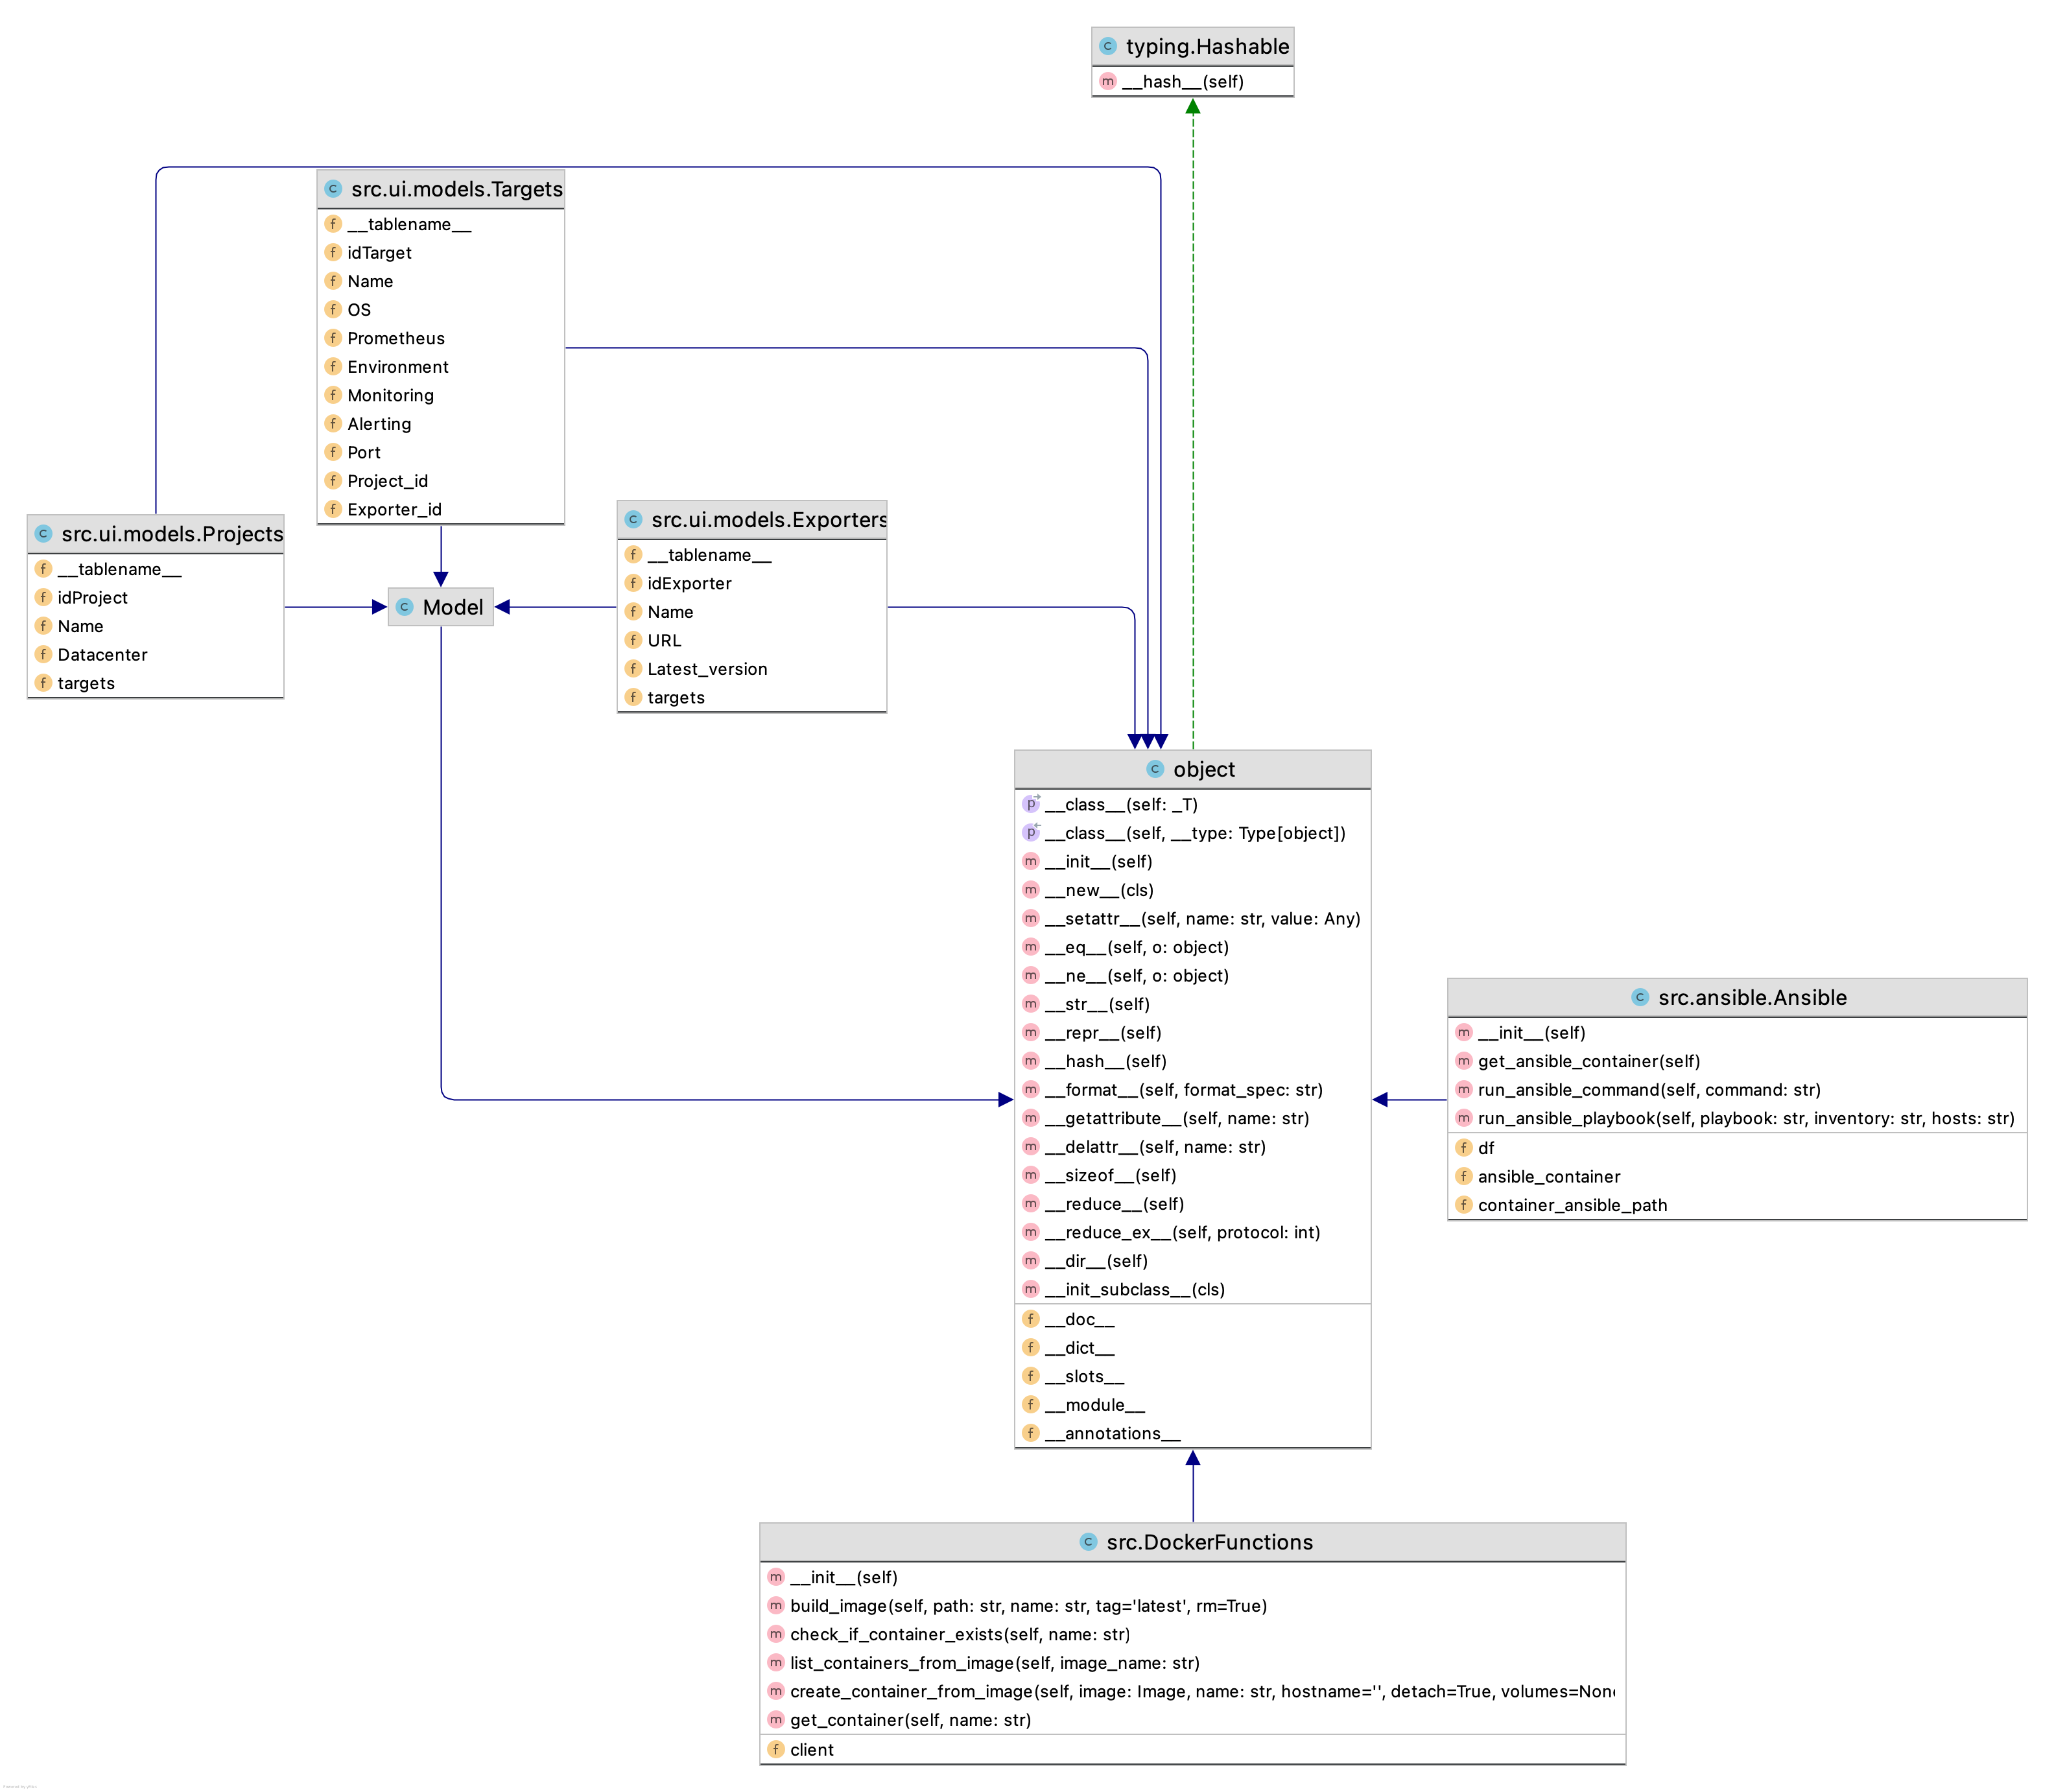
\includegraphics[width=0.9\textwidth]{include/desarrollo/src.png}
        \caption{Diagrama UML del backend}
        \label{fig:uml}
    \end{figure}
\end{center}

\section*{Ansible}
\label{sec:appendix_ansible}
\begin{lstlisting}[language=yaml,caption={Playbook creado para instalar \textit{node\_exporter}},label=lst:playbook]
- name: Install and start Node Exporter
  hosts: node_exporter
  tasks:
    - name: Create node_exporter dir
      become: yes
      file:
        path: '/opt/exporters/node_exporter'
        state: directory
        owner: root
        group: root
    - name: Install node exporter
      become: yes
      import_role:
        name: cloudalchemy.node_exporter
      vars:
        node_exporter_version: latest
        node_exporter_web_listen_address: "0.0.0.0:9100"
        node_exporter_web_telemetry_path: "/metrics"
        node_exporter_textfile_dir: "/opt/exporters/node_exporter/textfile_collector"
        node_exporter_enabled_collectors:
          - systemd
          - textfile:
              directory: "{{ node_exporter_textfile_dir }}"
        #  - filesystem:
        #      ignored-mount-points: "^/(sys|proc|dev)($|/)"
        #      ignored-fs-types: "^(sys|proc|auto)fs$"
        node_exporter_disabled_collectors: [ ]
        # Internal variables.
        _node_exporter_binary_install_dir: "/opt/exporters/node_exporter"
        _node_exporter_system_group: "prometheus"
        _node_exporter_system_user: "{{ _node_exporter_system_group }}"
\end{lstlisting}

\section*{Interfaz Gráfica}
\label{sec:appendix_gui}
\begin{figure}[H]
    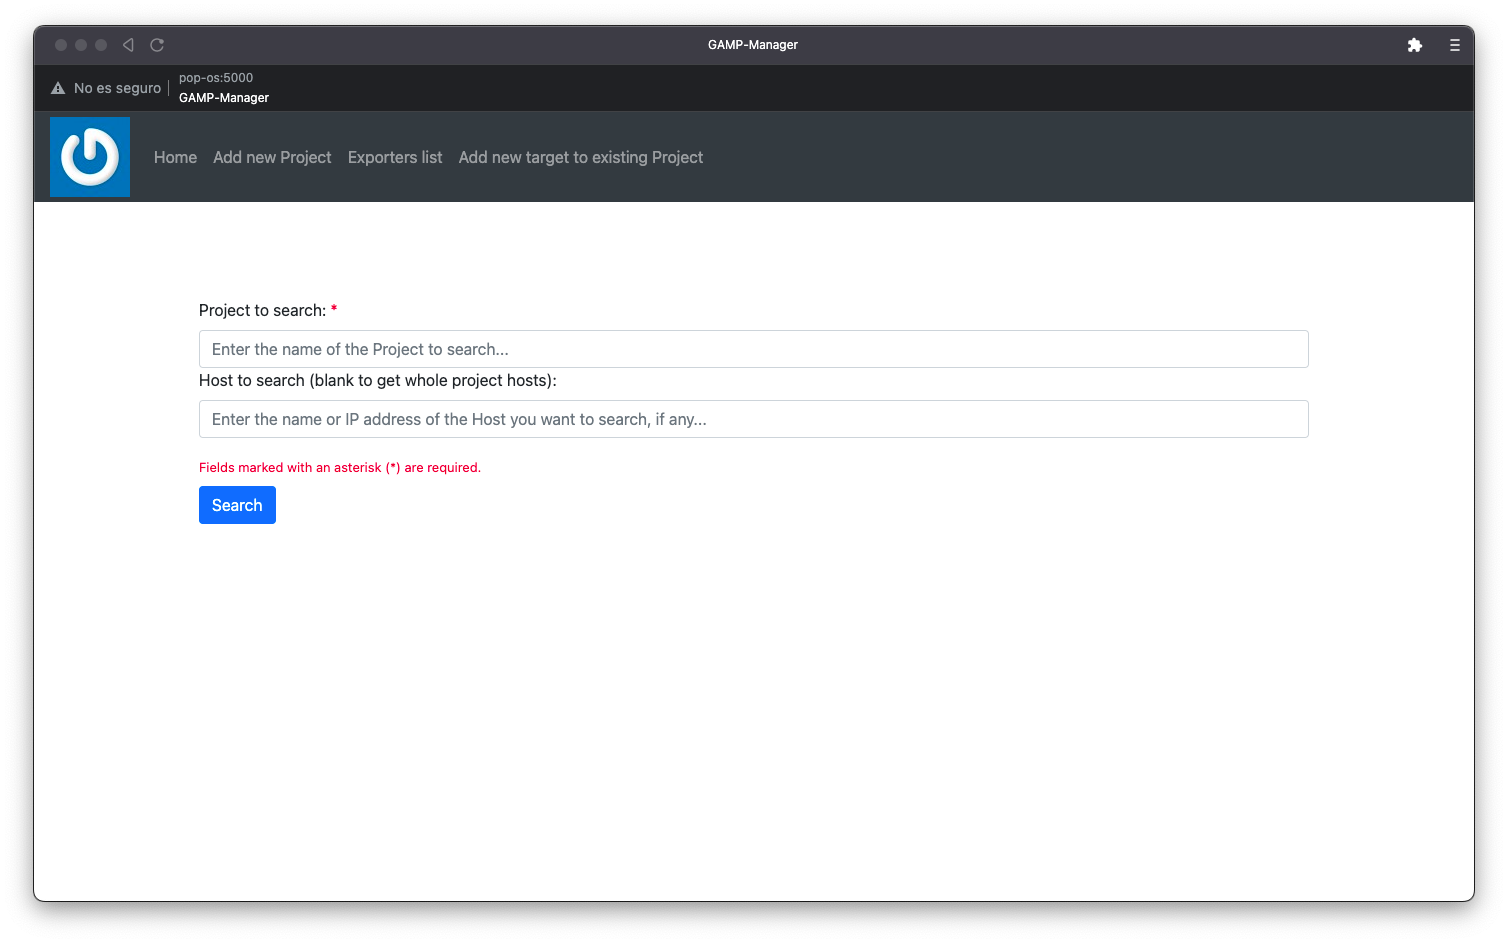
\includegraphics[width=\textwidth]{include/desarrollo/app_images/home.png}
    \caption{Página principal de selección de proyectos}
    \label{fig:gui_home}
\end{figure}

\begin{figure}[H]
    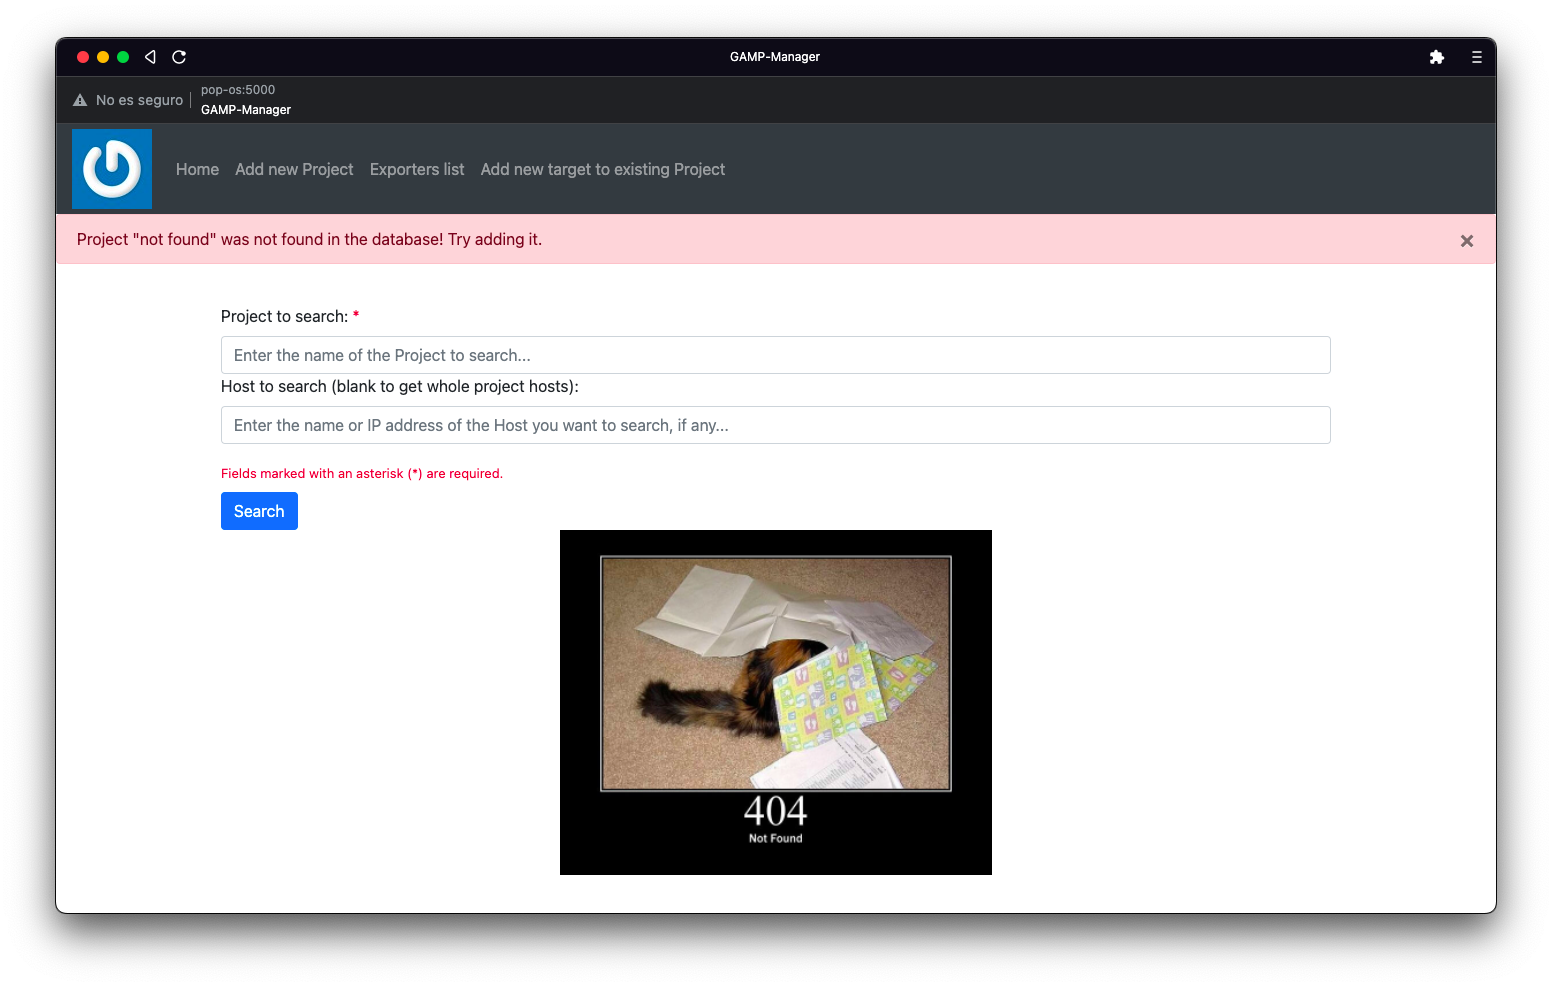
\includegraphics[width=\textwidth]{include/desarrollo/app_images/project_not_found.png}
    \caption{Proyecto no encontrado en la base de datos}
    \label{fig:gui_project_not_found}
\end{figure}

\begin{figure}[H]
    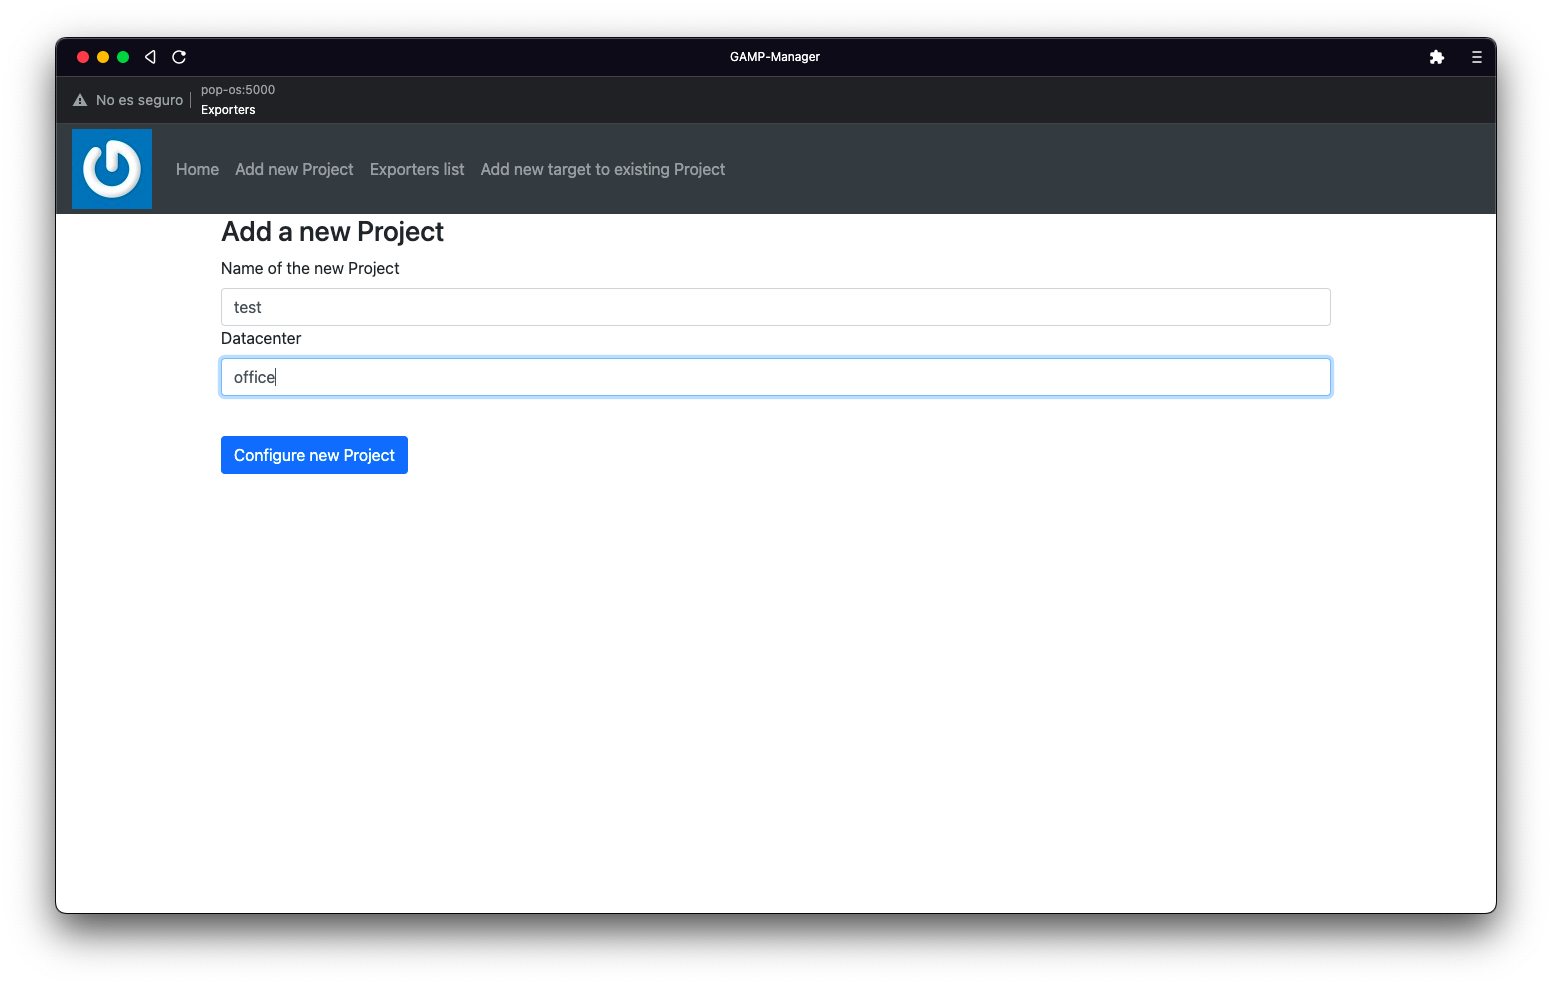
\includegraphics[width=\textwidth]{include/desarrollo/app_images/create_project.png}
    \caption{Creación de un proyecto nuevo}
    \label{fig:gui_create_project}
\end{figure}

\begin{figure}[H]
    \setbox1=\hbox{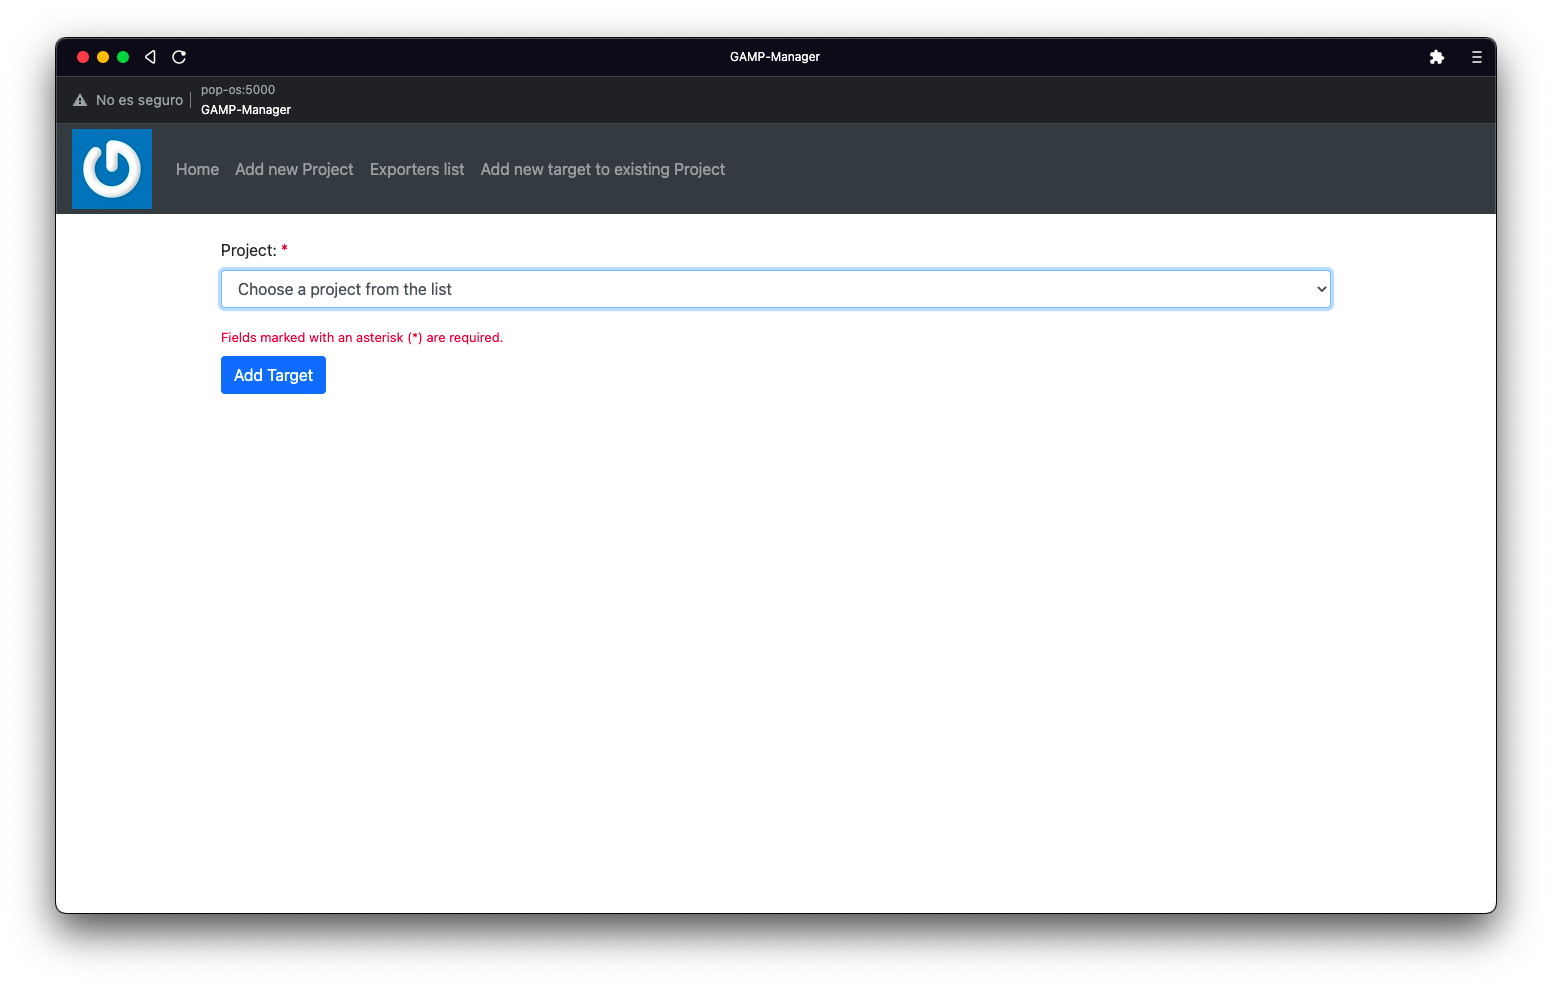
\includegraphics[width=\textwidth]{include/desarrollo/app_images/add_target_choose_project.png}}
    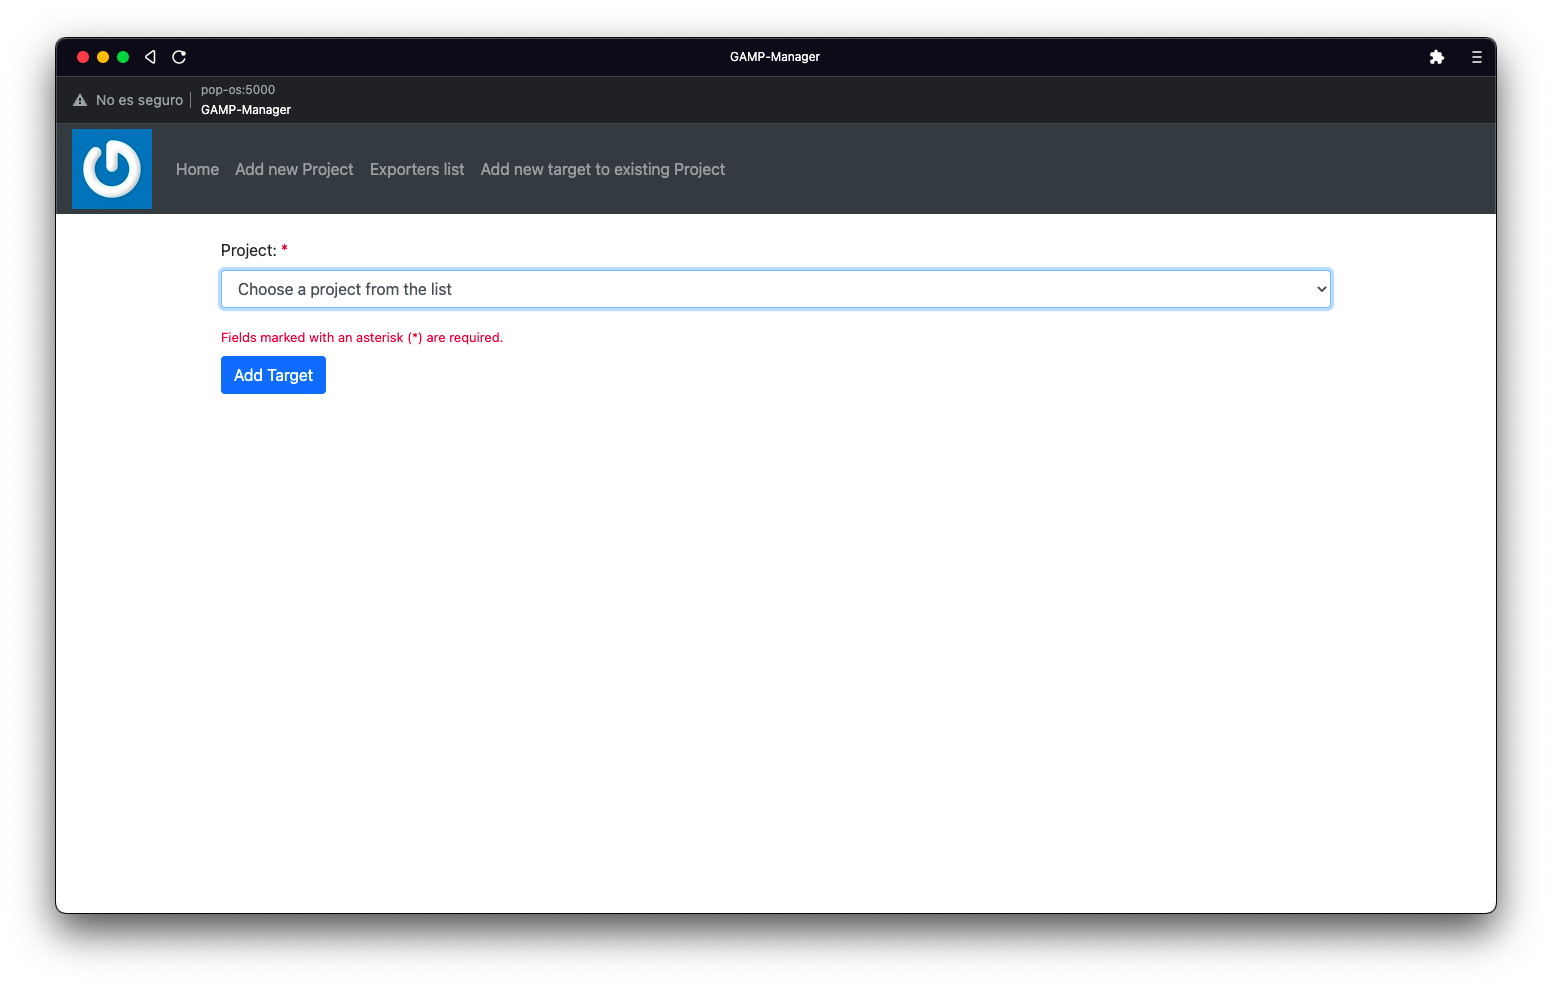
\includegraphics[width=\textwidth]{include/desarrollo/app_images/add_target_choose_project.png}\llap{\makebox[\wd1][c]{\raisebox{5.85cm}{\shifttext{-2.5cm}{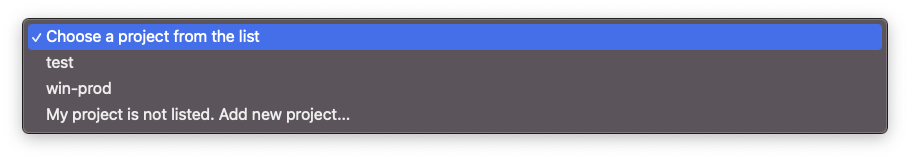
\includegraphics[width=0.6\textwidth]{include/desarrollo/app_images/project_list.png}}}}}
    \caption{Elección de proyecto para añadir	\textit{targets}}
    \label{fig:gui_add_target_choose_project}
\end{figure}

\begin{figure}[H]
    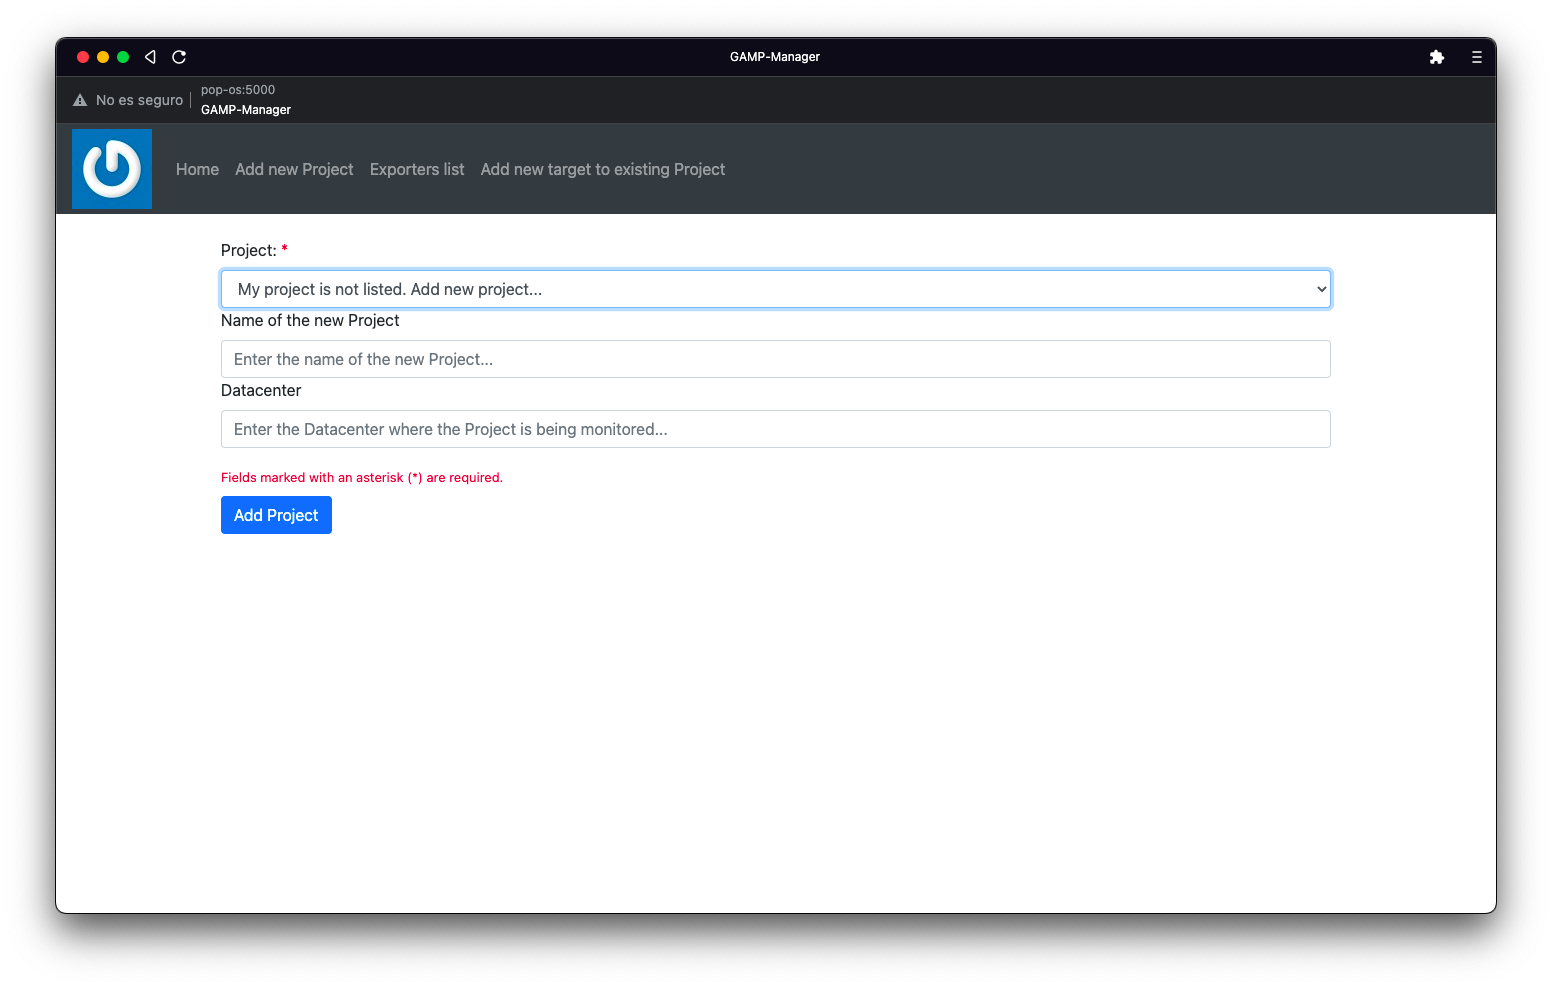
\includegraphics[width=\textwidth]{include/desarrollo/app_images/add_target_project_not_listed.png}
    \caption{Creación de un nuevo proyecto al intentar añadir	\textit{targets}}
    \label{fig:gui_add_target_project_not_listed}
\end{figure}

\begin{figure}[H]
    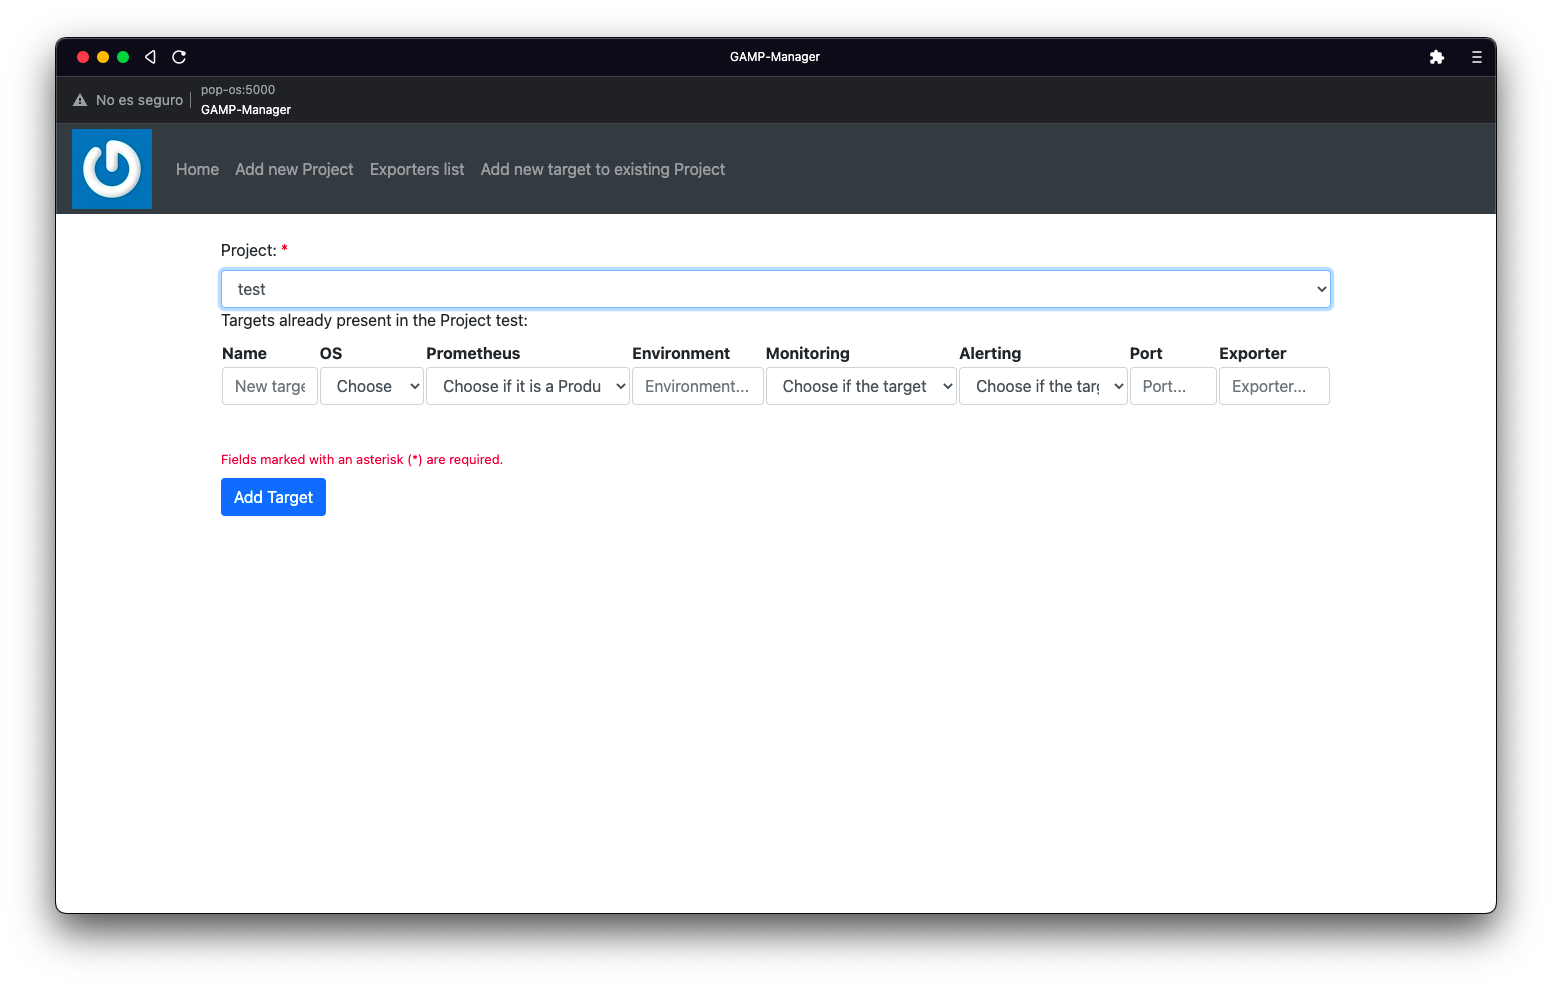
\includegraphics[width=\textwidth]{include/desarrollo/app_images/add_target_test.png}
    \caption{Creación de un target en un proyecto existente}
    \label{fig:gui_add_target_test}
\end{figure}

%%---------------------------------------------------------
\end{document}
